\chapter[Avaliação de modelos]{Avaliação de Modelos}

\begin{objetivos}
	Ao final deste capítulo, o leitor deverá ser capaz de:
	\begin{itemize}
		\item distinguir ajuste, discriminação, calibração e capacidade de transferência;
		\item explicar por que partições aleatórias podem produzir avaliações otimistas;
		\item escolher entre validação aleatória, espacial, ambiental e independente;
		\item interpretar AUC, TSS, Kappa, sensibilidade, especificidade e Boyce Index;
		\item avaliar criticamente limiares e mapas binários;
		\item comparar modelos sem reduzir a decisão a um ranking de métricas.
	\end{itemize}
\end{objetivos}

\section{Introdução}

A avaliação de modelos é uma etapa essencial em Modelagem de Distribuição de Espécies. Um modelo pode produzir mapas visualmente plausíveis, mas ainda assim apresentar baixa capacidade de discriminação, baixa sensibilidade, baixa especificidade ou forte dependência do conjunto de calibração. Por isso, modelos de SDM devem ser avaliados com dados independentes sempre que possível \parencite{fielding1997review,allouche2006assessing,hirzel2006evaluating,li2013thresholds,guisan2017habitat}.

Nesta unidade, a avaliação será aplicada ao fluxo real da apostila, comparando os modelos ajustados para \textit{Dinizia excelsa}: GLM, GAM, Random Forest, BRT, Maxent e Ensemble. O objetivo não é escolher automaticamente o modelo com maior métrica, mas compreender o desempenho, as limitações e a coerência ecológica de cada abordagem.

\begin{conceito}[title={\faBook\quad Avaliação não é apenas ranqueamento}]
	A avaliação de modelos não deve ser reduzida à escolha do maior AUC. Um modelo útil em SDM deve apresentar bom desempenho preditivo, coerência ecológica, respostas interpretáveis e capacidade de generalização espacial ou temporal.
\end{conceito}

\section{O que significa avaliar um SDM?}

Avaliar um modelo significa confrontar suas previsões com dados que não foram
usados para estimar seus parâmetros. Essa definição simples esconde quatro
perguntas diferentes. O modelo separa locais com presença de locais sem presença
ou de background? Os valores previstos são compatíveis com frequências
observadas quando possuem interpretação probabilística? O erro permanece
aceitável em outra região, período ou domínio ambiental? E a estratégia de teste
representa o uso que será feito do modelo?

Essas perguntas correspondem, respectivamente, a \textbf{discriminação},
\textbf{calibração}, \textbf{transferibilidade} e \textbf{adequação entre o
desenho de validação e o objetivo preditivo}. Um modelo pode discriminar bem e
ser mal calibrado; também pode obter ótimo desempenho dentro da região de
calibração e falhar quando transferido para condições novas
\parencite{vaughan2005testing,jimenezvalverde2013discrimination,roberts2017crossvalidation}.

\begin{atencao}[title={\faExclamationTriangle\quad Adequabilidade não é automaticamente probabilidade}]
	A calibração probabilística só deve ser interpretada dessa forma quando a
	saída do modelo e o desenho amostral sustentarem uma estimativa de
	probabilidade de ocorrência ou ocupação. Scores de presença--background e
	índices de adequabilidade não se tornam probabilidades apenas porque variam
	entre zero e um.
\end{atencao}

\section{Validação aleatória e dependência espacial}

Na validação cruzada aleatória, registros próximos podem ser distribuídos entre
treino e teste. Como locais vizinhos frequentemente compartilham clima, solo,
história de amostragem e autocorrelação residual, o conjunto de teste deixa de
representar uma previsão verdadeiramente nova. O resultado pode ser uma
subestimação do erro e uma impressão excessivamente otimista de generalização
\parencite{roberts2017crossvalidation}.

Esse problema é especialmente importante para ocorrências amazônicas
concentradas ao longo de rios, estradas, cidades e áreas historicamente
inventariadas. Uma divisão aleatória não remove essa estrutura; ela pode apenas
reparti-la entre os dois conjuntos.

\begin{conceito}[title={\faBook\quad Leakage espacial}]
	Há \textit{leakage} espacial quando a informação disponível no conjunto de
	treino torna o conjunto de teste artificialmente fácil por proximidade,
	dependência ou compartilhamento de unidades amostrais. O registro de teste
	pode ser formalmente diferente e, ainda assim, não constituir informação
	independente.
\end{conceito}

\section{Estratégias de partição}

\subsection{Validação cruzada aleatória}

É útil para diagnosticar o ajuste dentro do domínio amostrado e para comparar
implementações sob uma partição comum. Não deve ser apresentada como evidência
suficiente de transferência espacial quando os dados são estruturados.

\subsection{Blocos espaciais}

O domínio geográfico é dividido em blocos, e blocos inteiros são atribuídos ao
treino ou ao teste. A dimensão dos blocos precisa ser coerente com a escala de
autocorrelação, a densidade das ocorrências e a distância sobre a qual se deseja
predizer. Blocos pequenos demais preservam dependência; blocos grandes demais
podem produzir poucos folds, conjuntos desequilibrados e alta variância da
estimativa de erro \parencite{roberts2017crossvalidation,valavi2019blockcv}.

\subsection{Buffering e separação por distância}

Buffers removem do treino registros próximos aos pontos de teste. Essa estratégia
é útil quando a pergunta exige distância mínima explícita entre calibração e
avaliação. O custo é reduzir o conjunto de treino e, em amostras pequenas,
aumentar a variabilidade entre folds.

\subsection{Bloqueio ambiental}

Registros são separados em grupos do espaço ambiental, por exemplo por
agrupamento de variáveis contínuas. Essa estratégia avalia a capacidade do
modelo de predizer combinações ambientais não representadas no treino. Ela não
substitui o bloqueio geográfico: responde a uma pergunta de transferência
diferente \parencite{valavi2019blockcv}.

\subsection{Validação independente}

Dados coletados em outra campanha, região ou período fornecem o teste mais
direto para o respectivo tipo de transferência, desde que sejam comparáveis em
definição, esforço amostral e detectabilidade. Independência geográfica, por si
só, não corrige diferenças de protocolo.

\begin{atencao}[title={\faExclamationTriangle\quad Não existe uma partição universalmente melhor}]
	A estratégia deve imitar o uso pretendido. Interpolação dentro de uma paisagem,
	transferência para outra região e projeção climática futura são problemas
	diferentes e exigem testes diferentes.
\end{atencao}

\section{Implementação reproduzível dos folds espaciais}

Na aplicação com \textit{Dinizia excelsa}, os registros de presença e background
são associados a uma grade em projeção métrica. Células inteiras, e não registros
isolados, são atribuídas aos folds. Antes do ajuste, deve-se verificar se todos os
folds contêm as duas classes e se a separação espacial representa a distância de
predição relevante.

\begin{rcode}
# Executar a partir da raiz do projeto
source("scripts/unidade12/09_criar_folds_espaciais.R")
source("scripts/unidade12/10_validacao_espacial_glm.R")
\end{rcode}

\rscriptref{scripts/unidade12/09_criar_folds_espaciais.R}

\rscriptref{scripts/unidade12/10_validacao_espacial_glm.R}

O primeiro script grava a tabela de folds, a grade espacial e um mapa diagnóstico.
O segundo recalcula a padronização dos preditores usando exclusivamente o treino,
reajusta o GLM em cada fold e produz AUC, TSS, sensibilidade, especificidade e
Brier por fold. Reutilizar médias e desvios calculados com todos os registros
constituiria uma forma de leakage de pré-processamento.

\begin{atencao}[title={\faExclamationTriangle\quad O tamanho do bloco não é um hiperparâmetro decorativo}]
	O valor inicial de 300 km é uma configuração explícita para diagnóstico, não
	uma recomendação universal. A análise final deve justificar essa distância com
	base na escala da pergunta, no padrão de amostragem, na autocorrelação e no
	horizonte de transferência.
\end{atencao}

\begin{figure}[htbp]
	\centering
	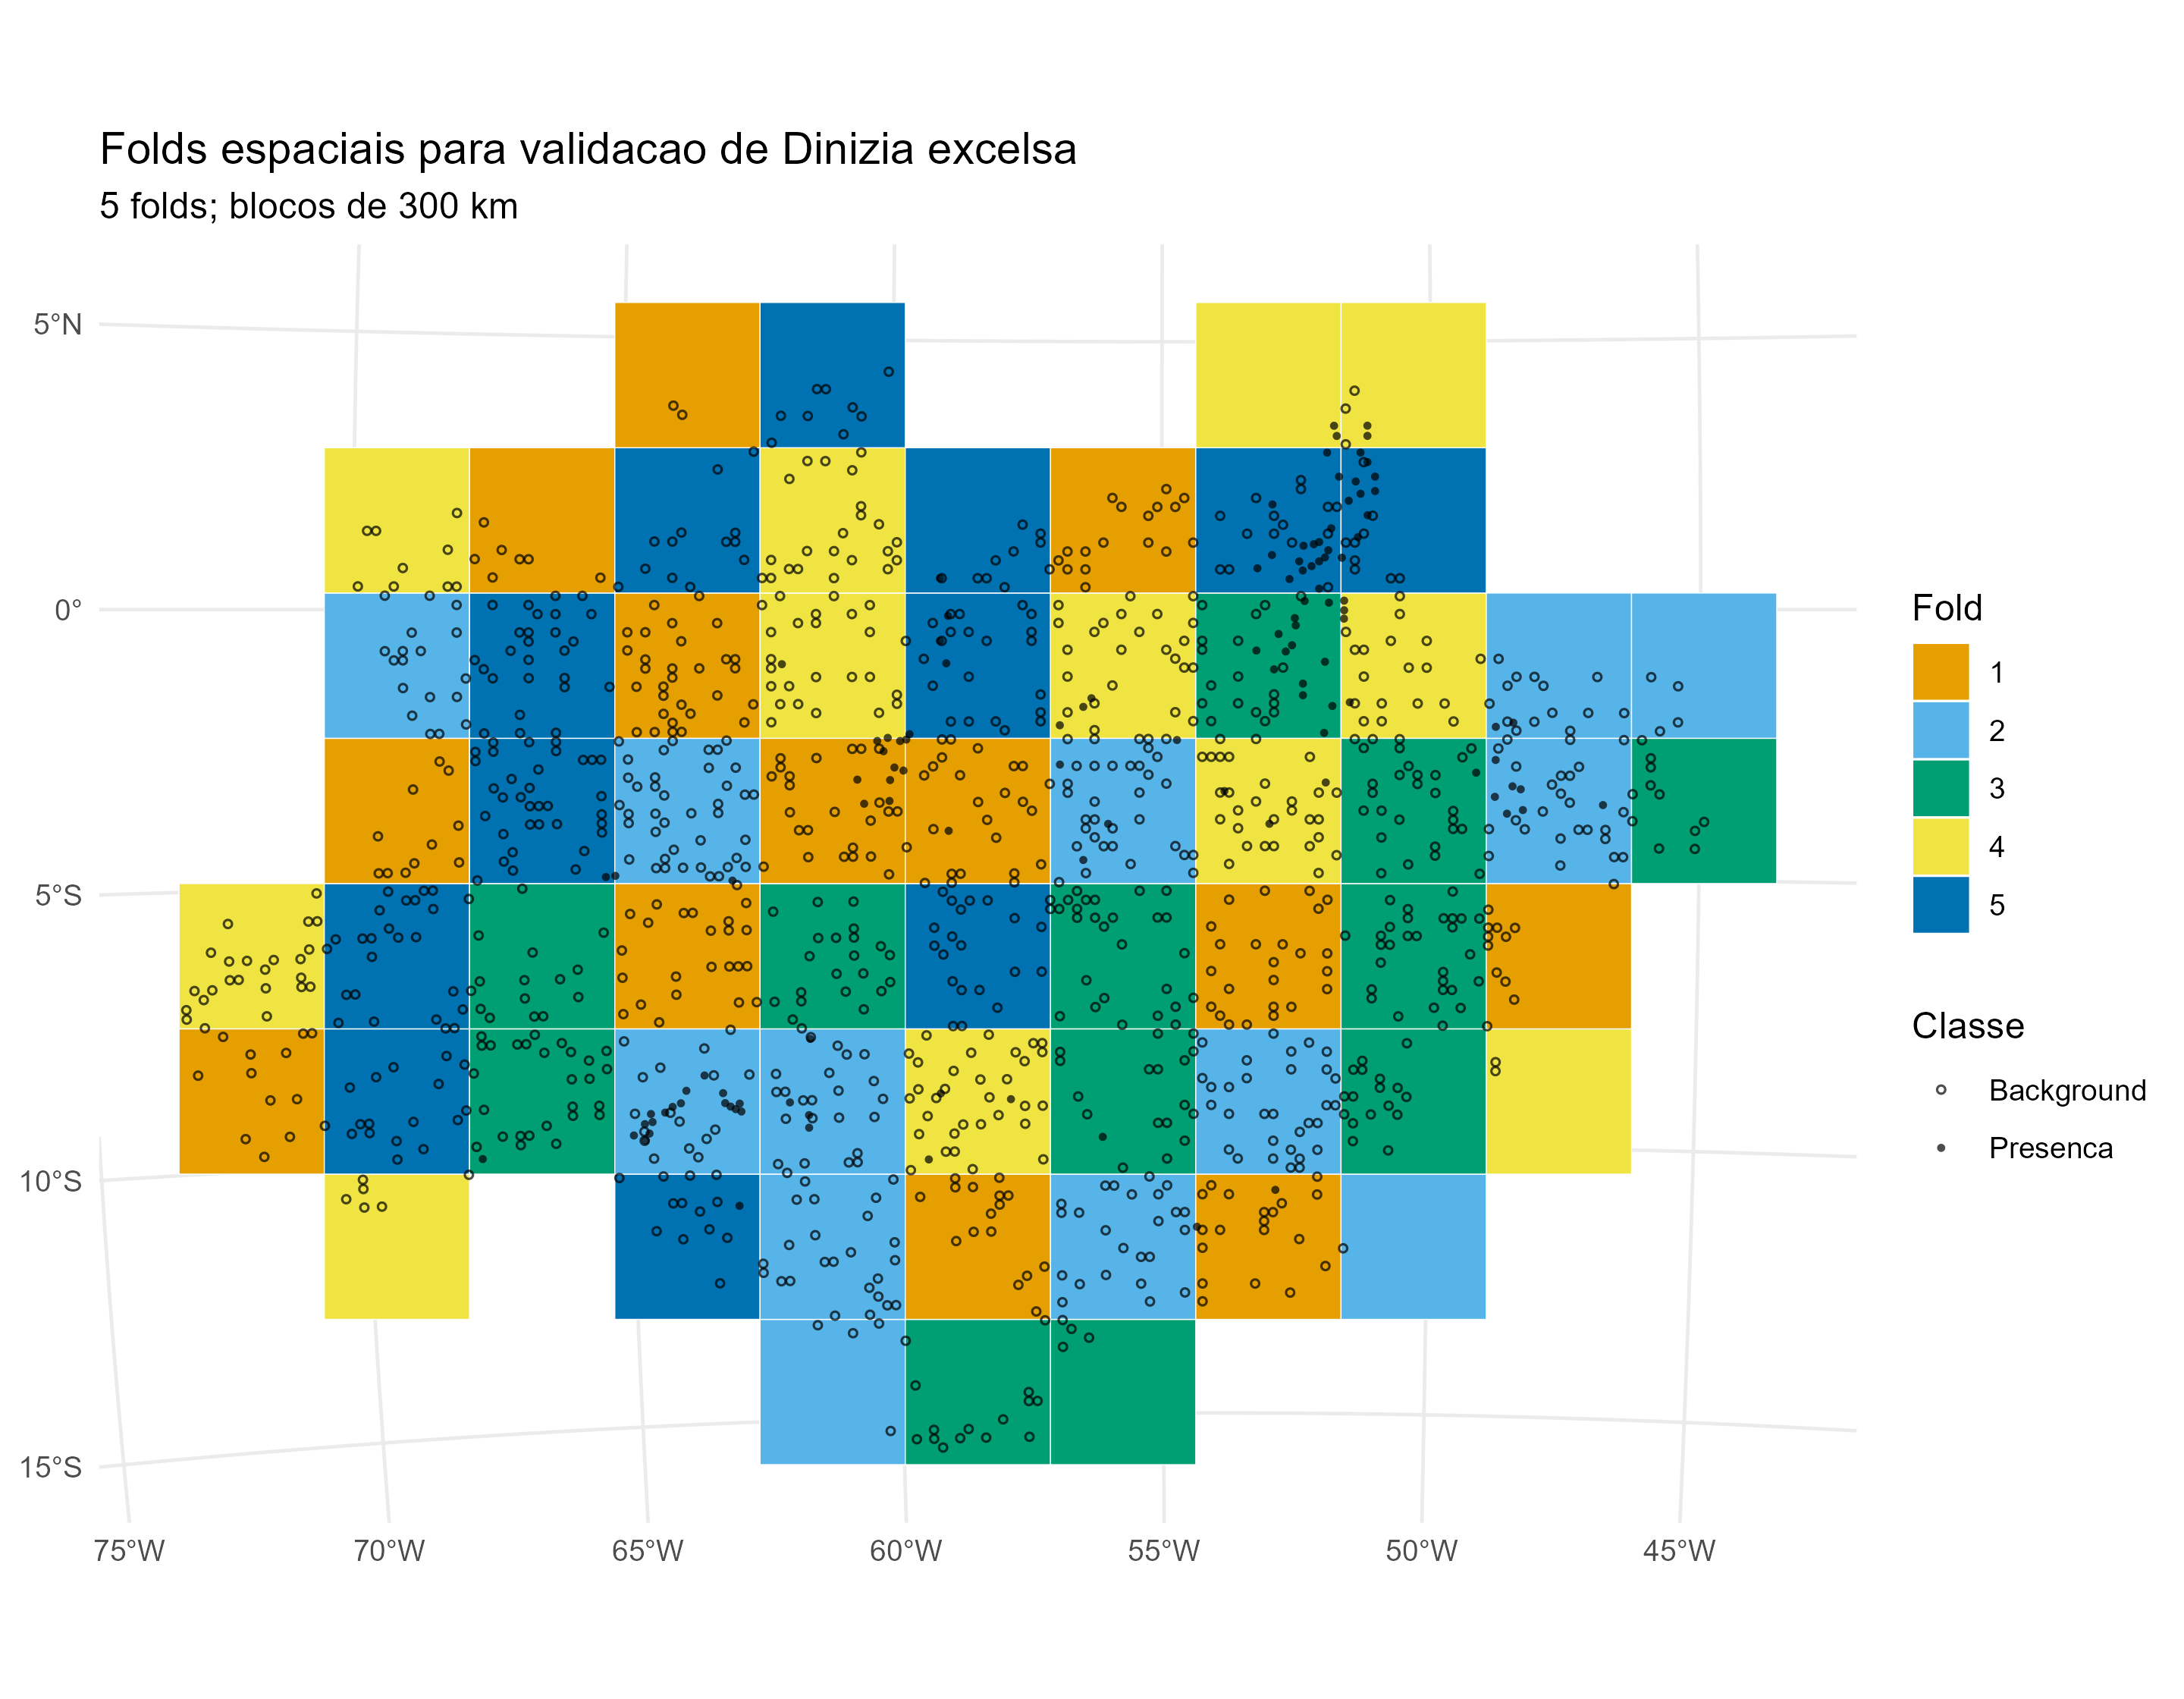
\includegraphics[width=0.93\textwidth]{figuras/unidade12/unidade12_folds_espaciais.png}
	\caption{Partição espacial reproduzível usada no diagnóstico. Cada célula de
	300 km pertence integralmente a um dos cinco folds; círculos preenchidos são
	presenças e círculos vazios são pontos de background. Células de um mesmo fold
	podem estar dispersas, portanto esta configuração não impõe uma faixa de
	exclusão entre treino e teste.}
	\label{fig:unidade12-folds-espaciais}
\end{figure}

\subsection{Resultado do diagnóstico espacial}

Todos os cinco folds retiveram presenças e background. O GLM convergiu nos cinco
reajustes, mas seu desempenho variou entre regiões: AUC foi de 0,643 a 0,851 e
especificidade de 0,475 a 0,829. Essa dispersão é mais informativa que um único
valor médio, pois revela onde a capacidade de transferência é menos estável.

\begin{table}[htbp]
	\centering
	\caption{Desempenho do GLM em cinco folds espaciais. Média e desvio-padrão
	(DP) resumem os reajustes independentes.}
	\label{tab:unidade12-validacao-espacial}
	\begin{tabular}{lrrr}
		\toprule
		Métrica & Média & DP & Amplitude \\
		\midrule
		AUC & 0,779 & 0,082 & 0,643--0,851 \\
		TSS & 0,528 & 0,093 & 0,419--0,658 \\
		Sensibilidade & 0,826 & 0,132 & 0,632--0,944 \\
		Especificidade & 0,703 & 0,155 & 0,475--0,829 \\
		Brier & 0,078 & 0,030 & 0,043--0,116 \\
		\bottomrule
	\end{tabular}
\end{table}

\begin{figure}[htbp]
	\centering
	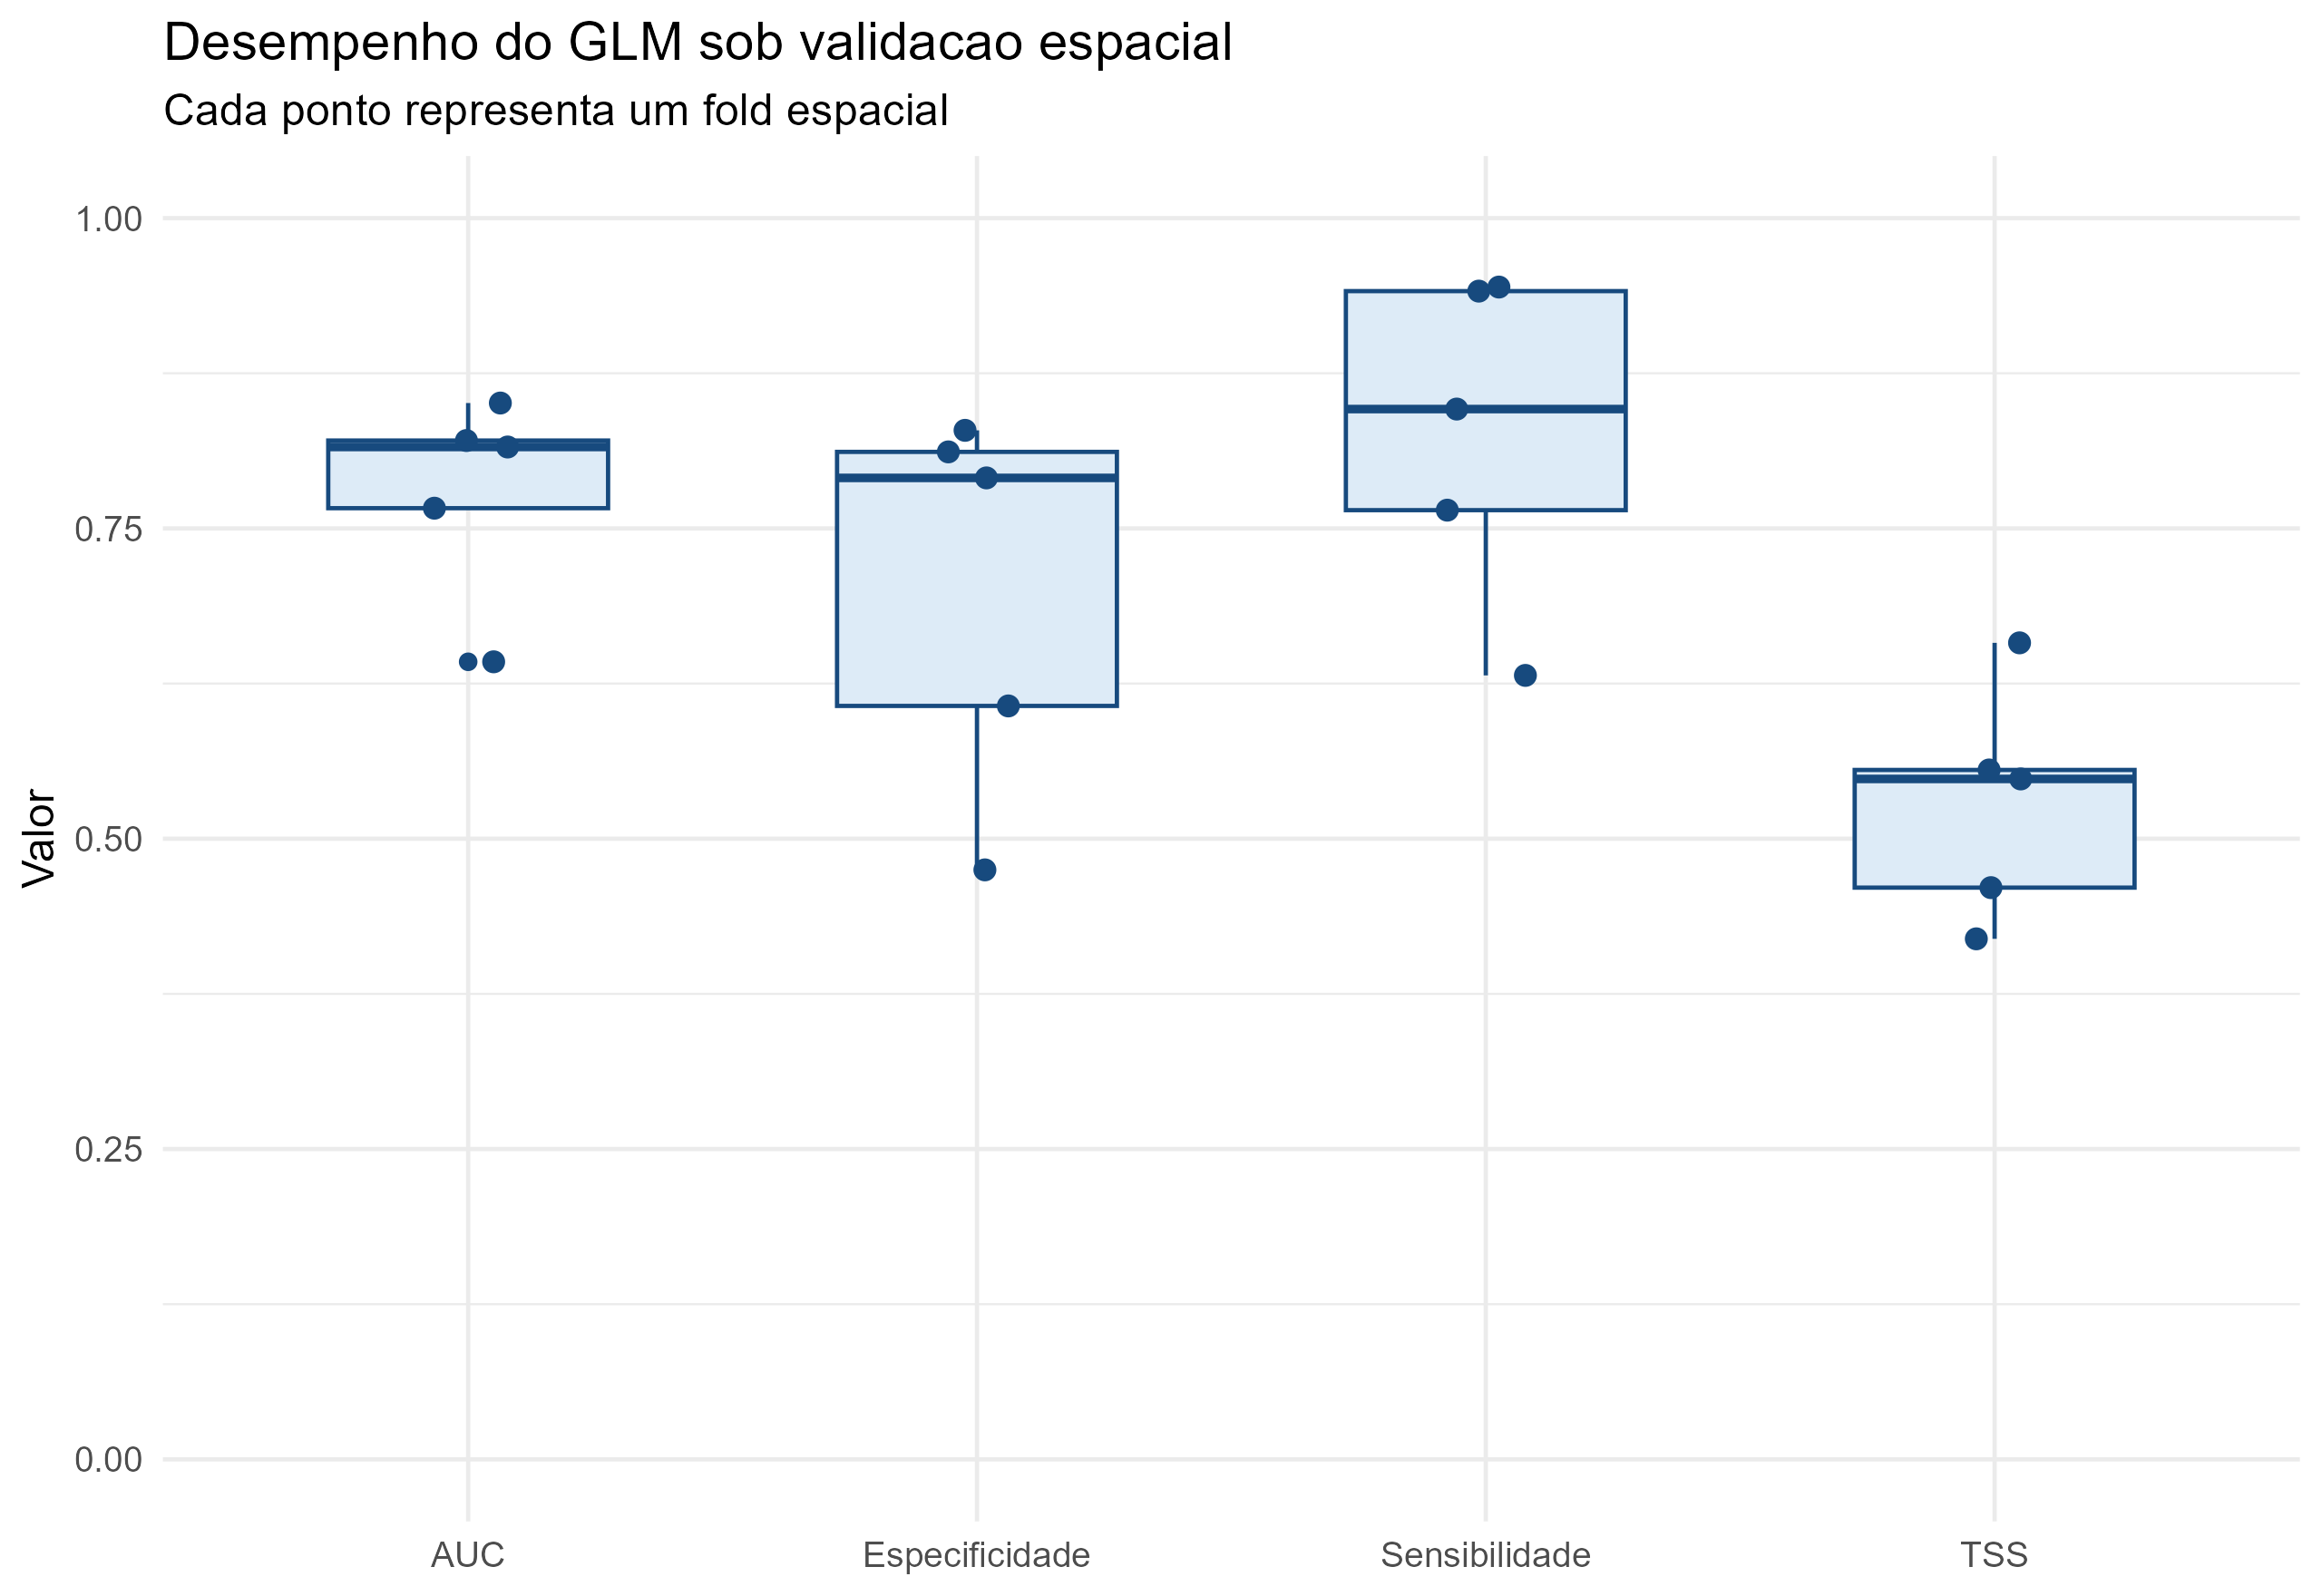
\includegraphics[width=0.88\textwidth]{figuras/unidade12/unidade12_validacao_espacial_glm.png}
	\caption{Variação das métricas do GLM entre os cinco folds espaciais. Os
	pontos são os resultados de cada fold; a caixa é apenas um resumo visual e
	não substitui a inspeção dos valores individuais.}
	\label{fig:unidade12-desempenho-espacial}
\end{figure}

Os ajustes emitiram avisos de probabilidades numericamente próximas de zero ou
um. Embora todos tenham convergido, 37 previsões de teste foram extremas pelo
critério operacional \(\hat p \leq 10^{-6}\) ou
\(\hat p \geq 1-10^{-6}\). Isso pode indicar separação, extrapolação ou excesso
de flexibilidade dos termos quadráticos e deve ser investigado antes de tratar
os scores como probabilidades calibradas. Estes resultados não demonstram, por
si só, superioridade ou inferioridade em relação à validação aleatória: essa
comparação exigiria o mesmo modelo, dados, pré-processamento e métricas, alterando
somente o esquema de partição.

\section{Spatial sorting bias}

O \textit{spatial sorting bias} ocorre quando as presenças de teste estão, em
média, mais próximas das presenças de treino do que os pontos de ausência ou
background usados na avaliação. Nessa situação, até um modelo baseado somente
em distância geográfica pode obter AUC elevado. A inspeção das distâncias entre
treino e teste e a comparação com modelos nulos ajudam a revelar esse viés
\parencite{hijmans2012spatialsorting}.

\begin{decisao}[title={\faRoute\quad Decisão metodológica}]
	Antes de calcular métricas, declare qual capacidade está sendo testada:
	interpolação local, transferência geográfica, transferência ambiental ou
	projeção temporal. Em seguida, construa folds que representem essa distância
	de previsão e mantenha os mesmos folds na comparação entre algoritmos.
\end{decisao}

\section{Discriminação e calibração}

Discriminação descreve a ordenação relativa dos casos: presenças recebem scores
maiores que ausências ou background? Calibração descreve a correspondência entre
valores previstos e frequências observadas, quando essa interpretação é válida.
Curvas ROC e AUC avaliam discriminação, não calibração. Diagramas de confiabilidade,
intercepto e inclinação de calibração e escores próprios podem complementar a
avaliação de modelos probabilísticos \parencite{vaughan2005testing,jimenezvalverde2013discrimination}.

\begin{conceito}[title={\faBalanceScale\quad Um modelo pode acertar a ordem e errar a magnitude}]
	Dois modelos podem ordenar os locais de modo semelhante e apresentar AUC
	parecido, mas produzir valores com significados e calibração muito diferentes.
Por isso, bom desempenho discriminatório não autoriza interpretar adequabilidade
como probabilidade de ocorrência.
\end{conceito}

\section{AUC e curva ROC}

A curva ROC representa a relação entre sensibilidade e \(1 -\) especificidade ao longo de diferentes limiares. A área sob a curva, ou AUC, mede a capacidade do modelo de discriminar presenças de background ou ausências.

\begin{equationbox}
	\[
	AUC = P(\hat{y}_{presença} > \hat{y}_{background})
	\]
\end{equationbox}

Em termos intuitivos, AUC representa a probabilidade de uma presença receber valor de adequabilidade maior que um ponto de background escolhido aleatoriamente.

\begin{atencao}[title={\faExclamationTriangle\quad Limitações do AUC}]
	Em dados presença-background, AUC pode ser influenciado pela extensão geográfica, pelo background escolhido, pelo viés amostral e pela prevalência. Valores altos não garantem necessariamente bom modelo ecológico.
\end{atencao}

\section{Sensibilidade, especificidade e TSS}

A sensibilidade mede a proporção de presenças corretamente previstas como adequadas. A especificidade mede a proporção de backgrounds ou ausências corretamente classificadas como inadequadas.

\begin{equationbox}
	\[
	Sensibilidade = \frac{TP}{TP + FN}
	\]
	
	\[
	Especificidade = \frac{TN}{TN + FP}
	\]
	
	\[
	TSS = Sensibilidade + Especificidade - 1
	\]
\end{equationbox}

O TSS varia de \(-1\) a \(1\), sendo valores próximos de \(1\) indicativos de melhor discriminação binária.

\section{Kappa}

O índice Kappa mede o acordo entre predição binária e observação, corrigindo pelo acordo esperado ao acaso. Embora tenha sido amplamente utilizado em SDM, ele pode ser sensível à prevalência e à distribuição dos dados.

\begin{equationbox}
	\[
	Kappa = \frac{p_o - p_e}{1 - p_e}
	\]
\end{equationbox}

em que \(p_o\) é o acordo observado e \(p_e\) é o acordo esperado ao acaso.

\section{Boyce Index}

O Boyce Index é uma métrica especialmente útil para modelos presença-background ou presença-apenas. Ele avalia se as presenças tendem a ocorrer em áreas com maiores valores de adequabilidade previstos pelo modelo \parencite{hirzel2006evaluating}.

\begin{conceito}[title={\faBook\quad Boyce Index}]
	O Boyce Index mede a consistência entre adequabilidade prevista e frequência observada de presenças. Valores positivos indicam que as presenças se concentram em classes de maior adequabilidade.
\end{conceito}

\section{Preparação da avaliação integrada}

Nesta unidade, organizamos as predições de teste dos modelos individuais e do ensemble para construir uma avaliação comparativa.

\rscriptfile{scripts/unidade12/01_estrutura_pastas.R}

\rscriptfile{scripts/unidade12/02_preparar_predicoes_avaliacao.R}

\section{Cálculo das métricas}

\rscriptfile{scripts/unidade12/03_calcular_metricas_modelos.R}

\begin{figure}[H]
	\centering
	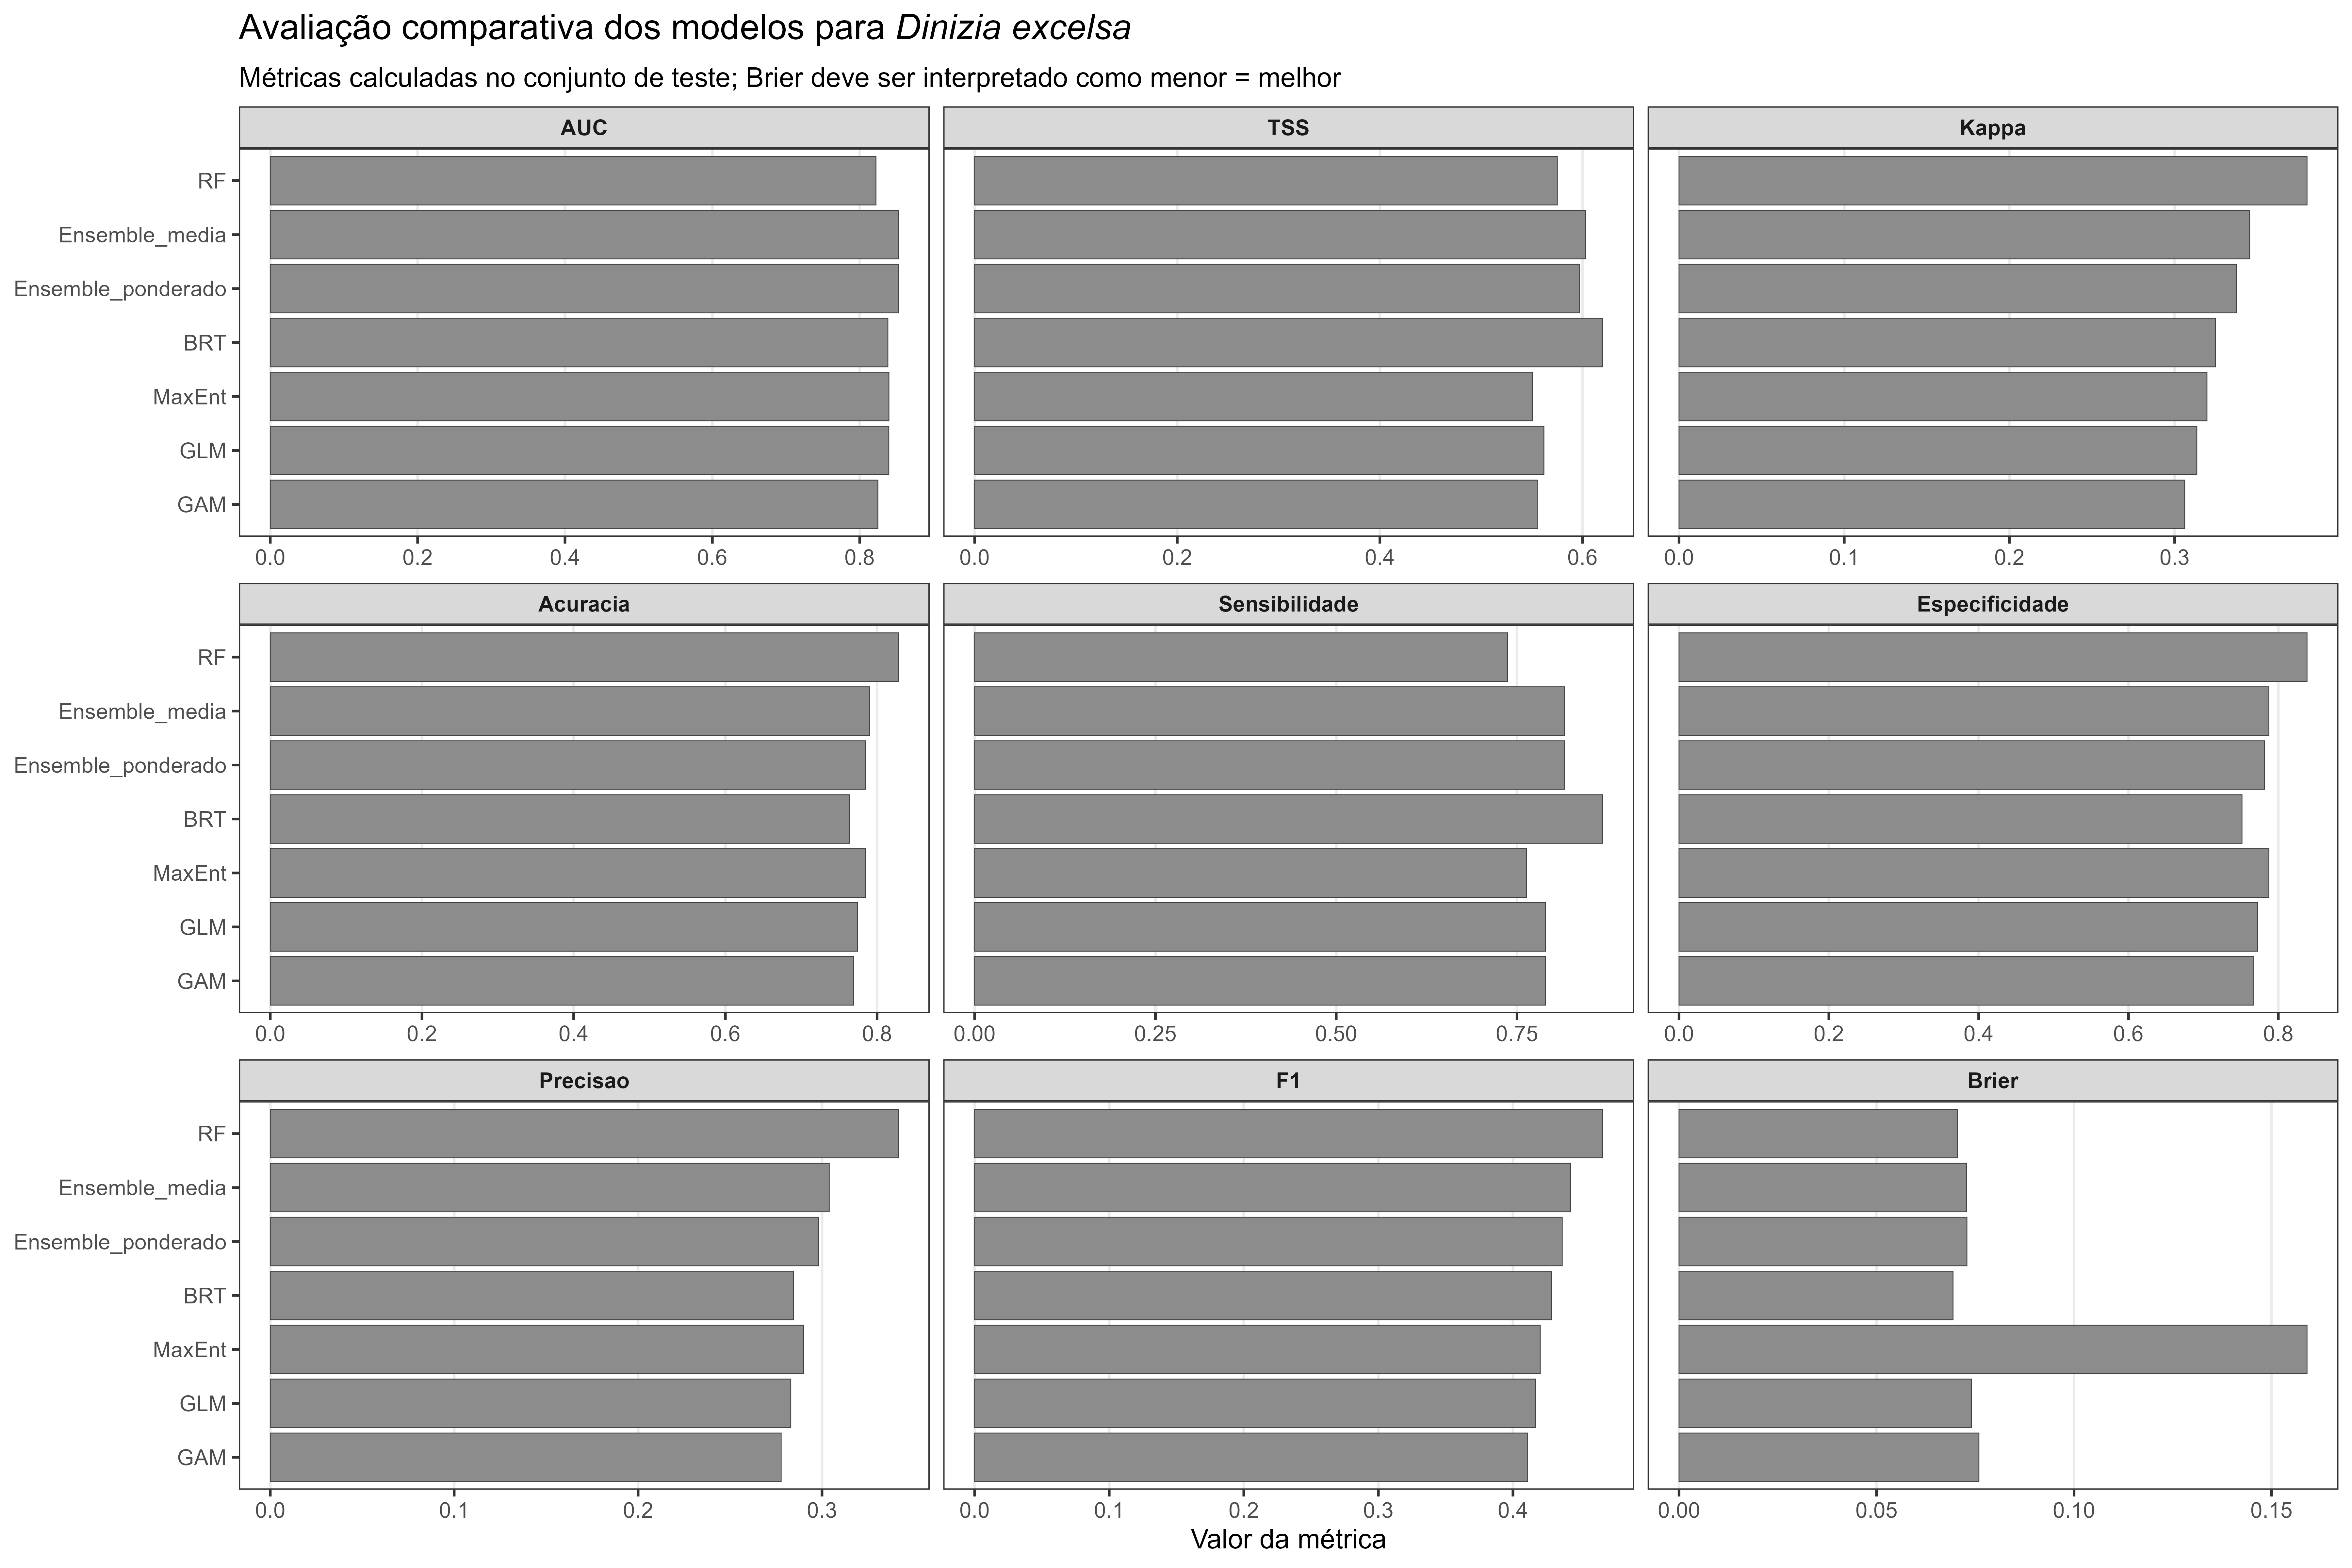
\includegraphics[width=0.95\textwidth]{figuras/unidade12/unidade12_comparacao_metricas.png}
	\caption{Comparação das métricas de avaliação dos modelos ajustados para \textit{Dinizia excelsa}.}
	\label{fig:unidade12_metricas}
\end{figure}

\section{Curvas ROC comparativas}

\rscriptfile{scripts/unidade12/04_curvas_roc_comparativas.R}

\begin{figure}[H]
	\centering
	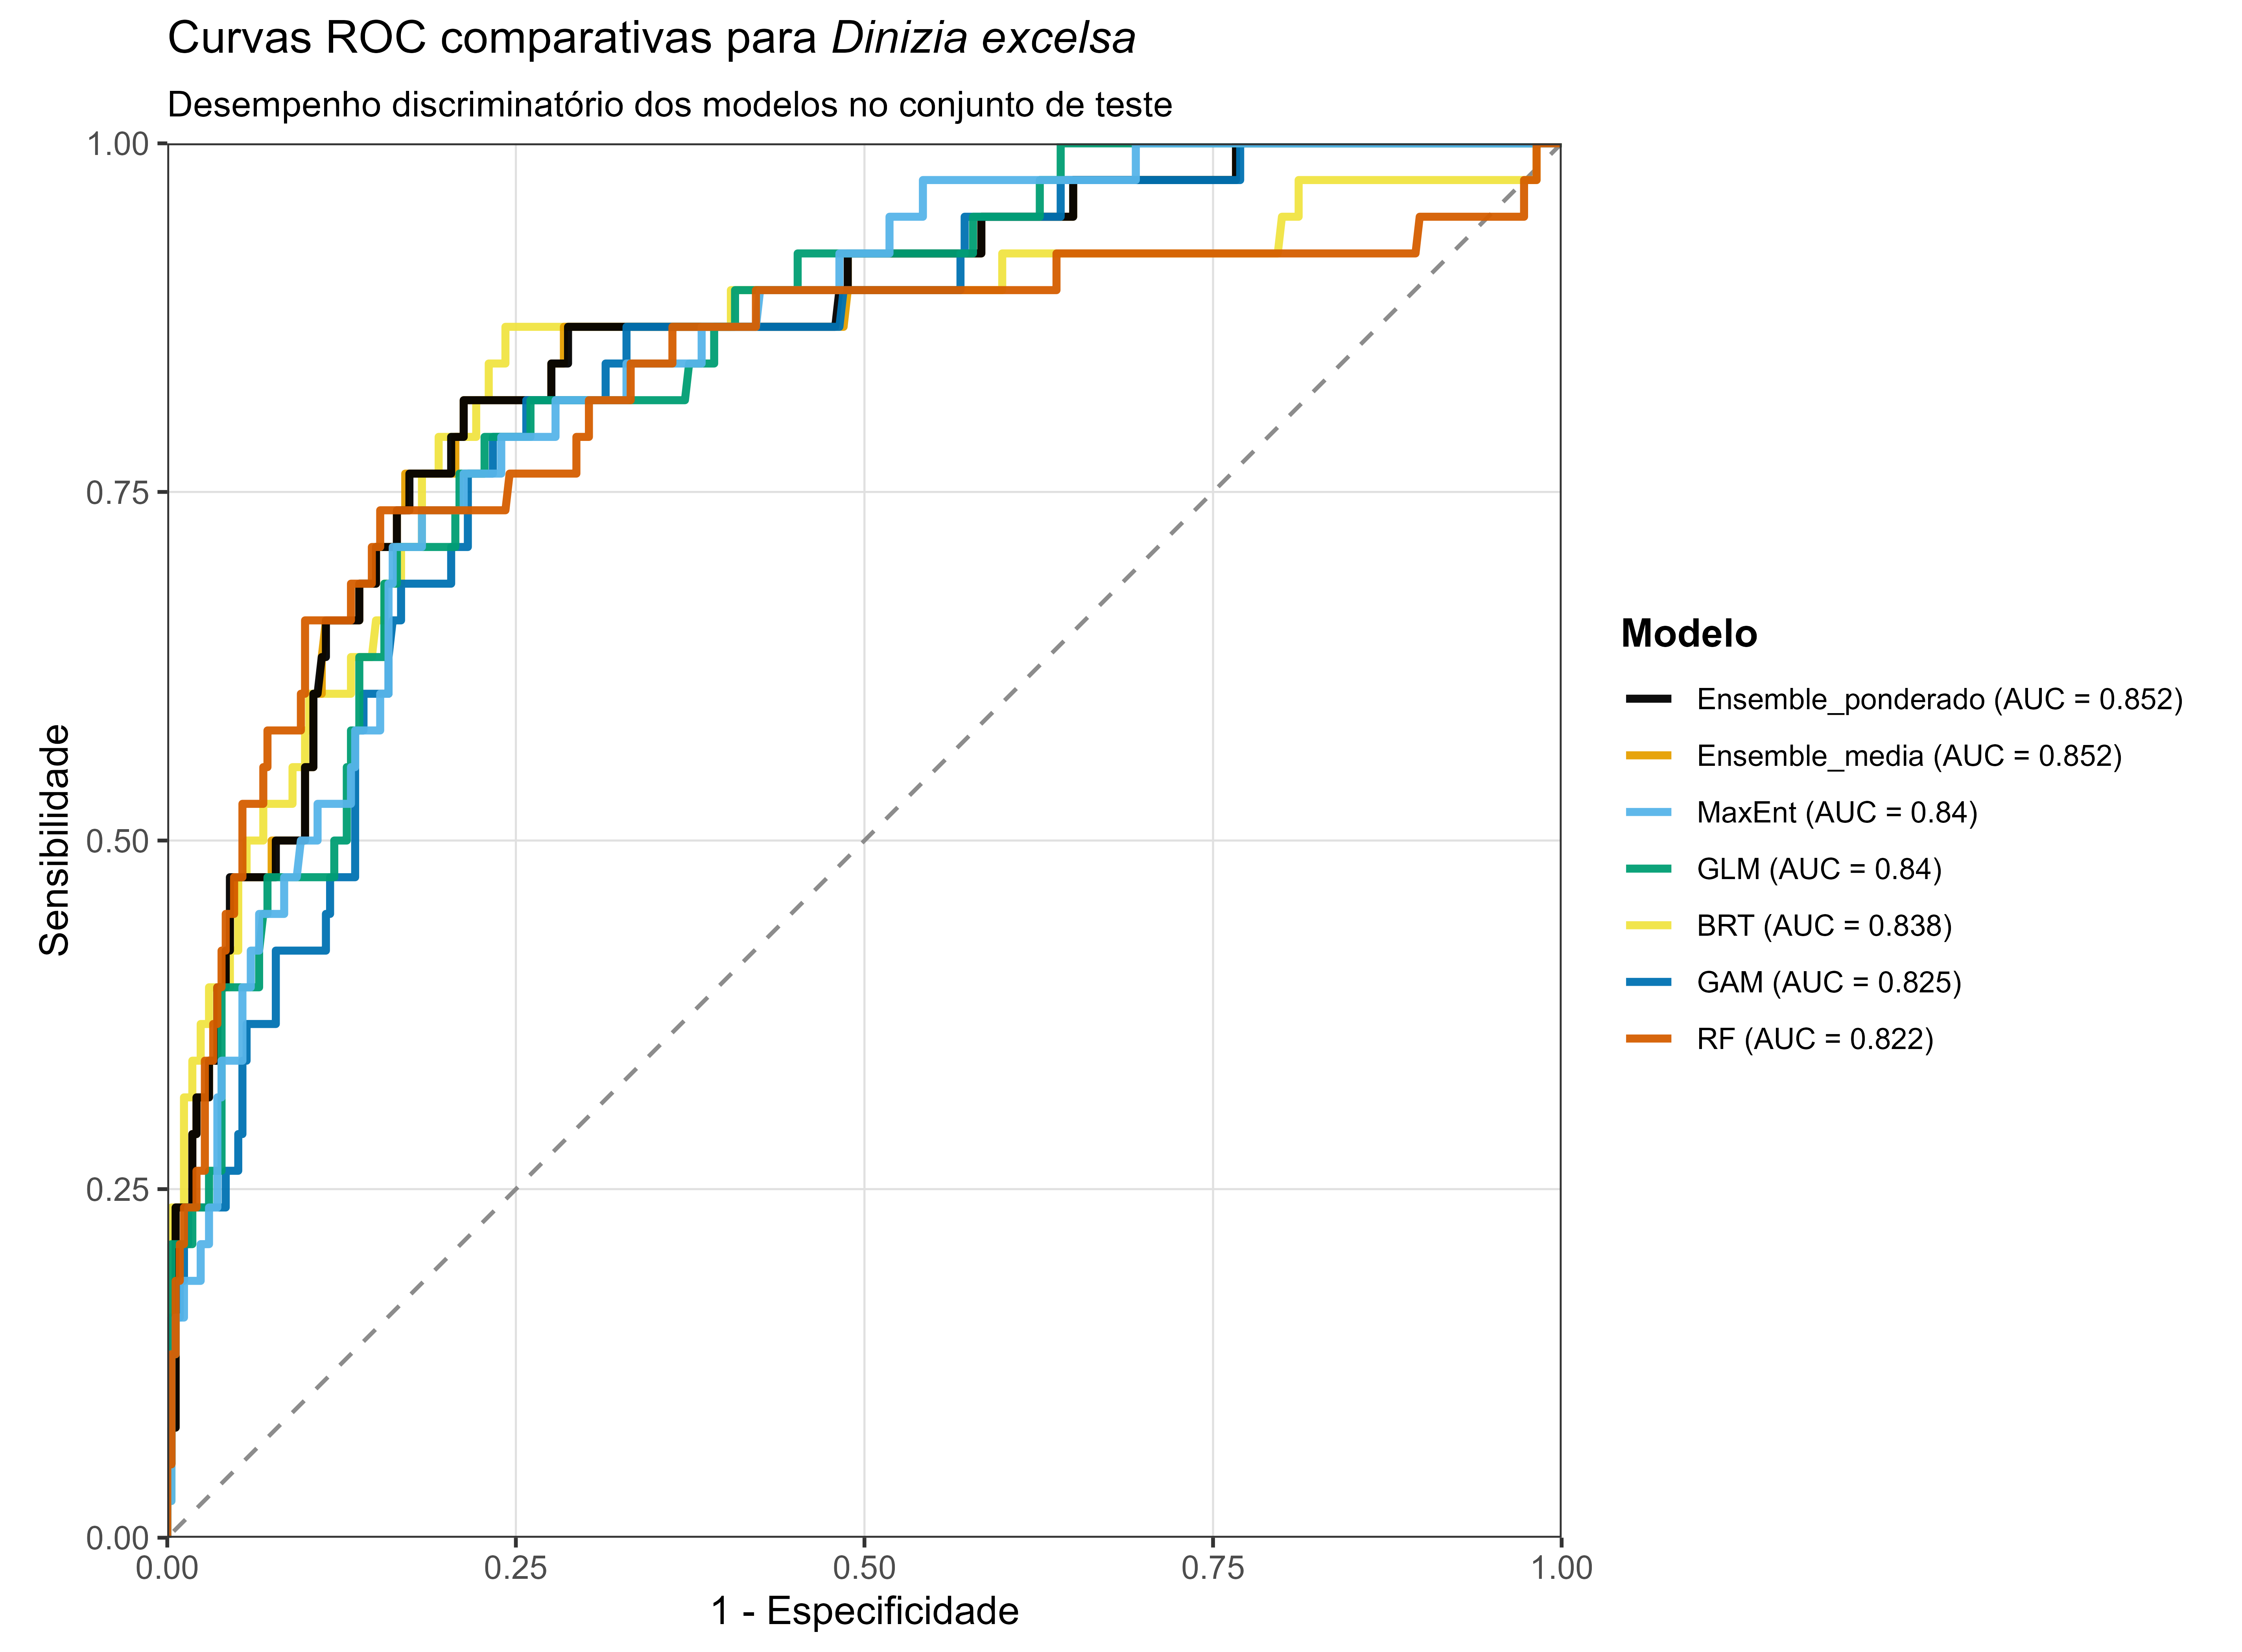
\includegraphics[width=0.86\textwidth]{figuras/unidade12/unidade12_curvas_roc_comparativas.png}
	\caption{Curvas ROC comparativas para GLM, GAM, Random Forest, BRT, Maxent e Ensemble.}
	\label{fig:unidade12_roc_comparativas}
\end{figure}

\section{Matrizes de confusão}

\rscriptfile{scripts/unidade12/05_matrizes_confusao.R}

\begin{figure}[H]
	\centering
	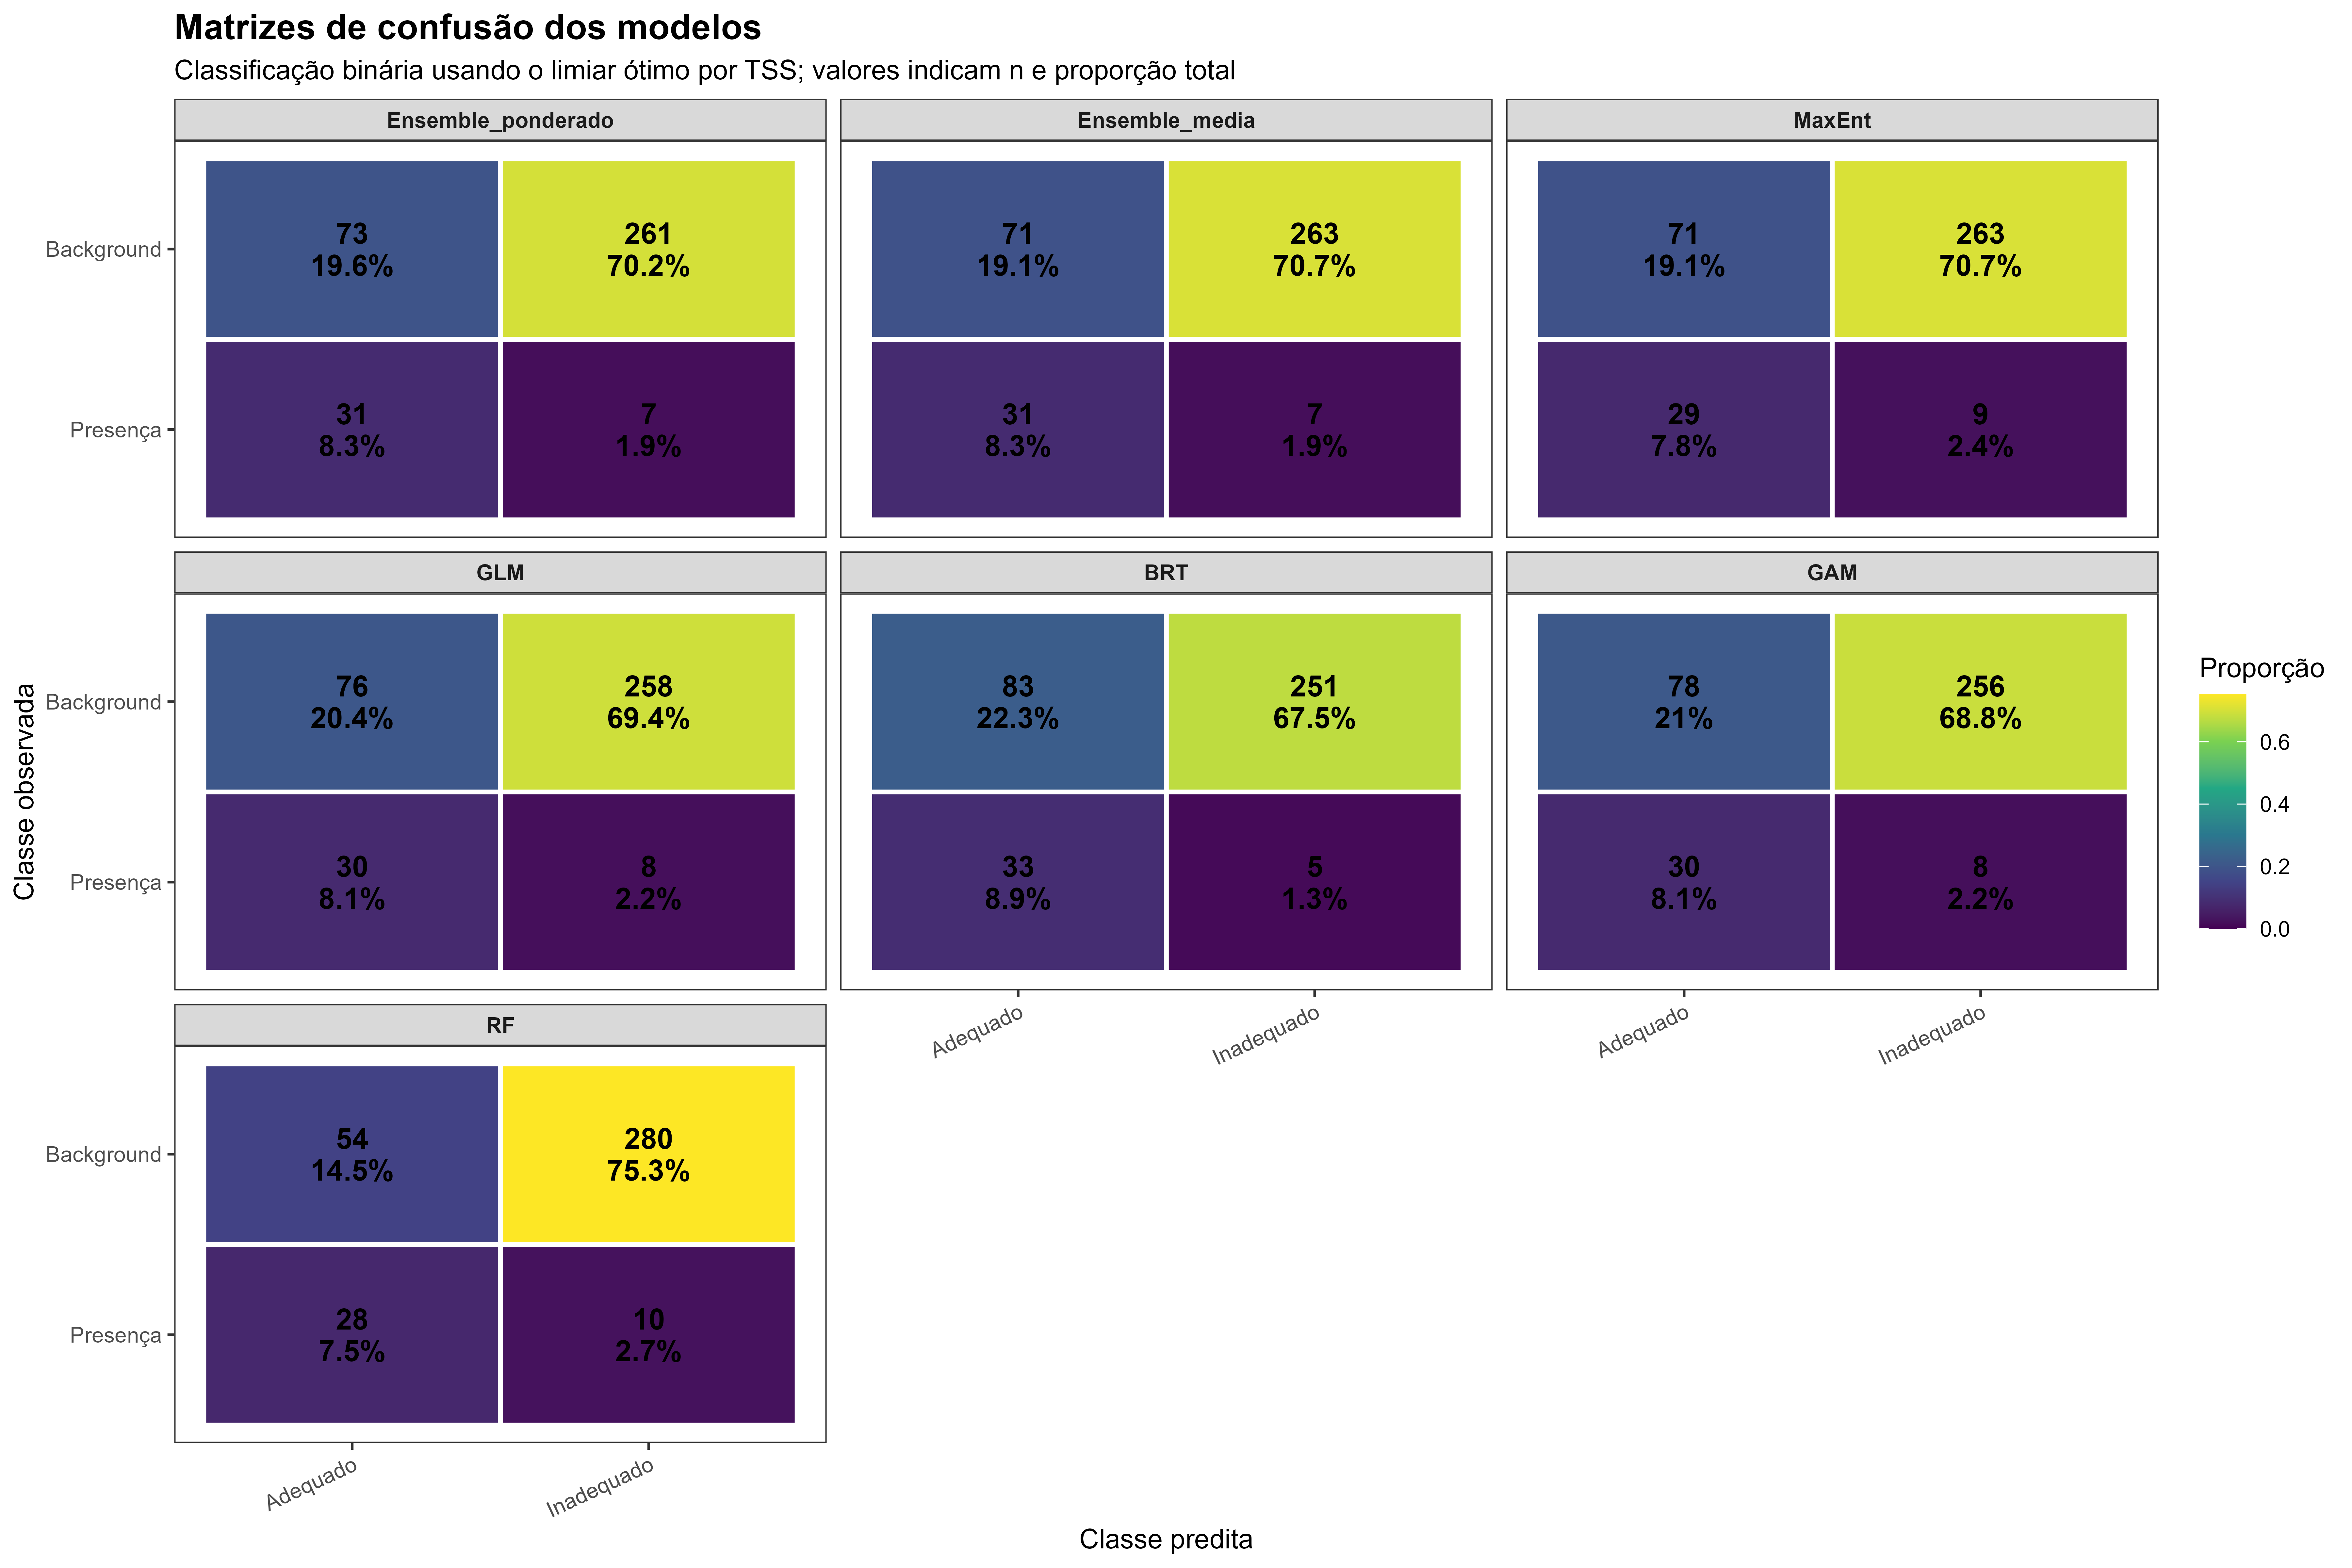
\includegraphics[width=0.95\textwidth]{figuras/unidade12/unidade12_matrizes_confusao.png}
	\caption{Matrizes de confusão dos modelos avaliados com limiares ótimos definidos pelo TSS.}
	\label{fig:unidade12_matrizes_confusao}
\end{figure}

\section{Mapas binários}

\rscriptfile{scripts/unidade12/06_mapas_binarios.R}

\begin{figure}[H]
	\centering
	\includegraphics[width=0.98\textwidth]{figuras/unidade12/unidade12_mapas_binarios.png}
	\caption{Mapas binários de adequabilidade ambiental para \textit{Dinizia excelsa}, gerados a partir dos limiares ótimos por TSS.}
	\label{fig:unidade12_mapas_binarios}
\end{figure}

\section{Síntese comparativa}

\rscriptfile{scripts/unidade12/07_sintese_avaliacao.R}

\begin{figure}[H]
	\centering
	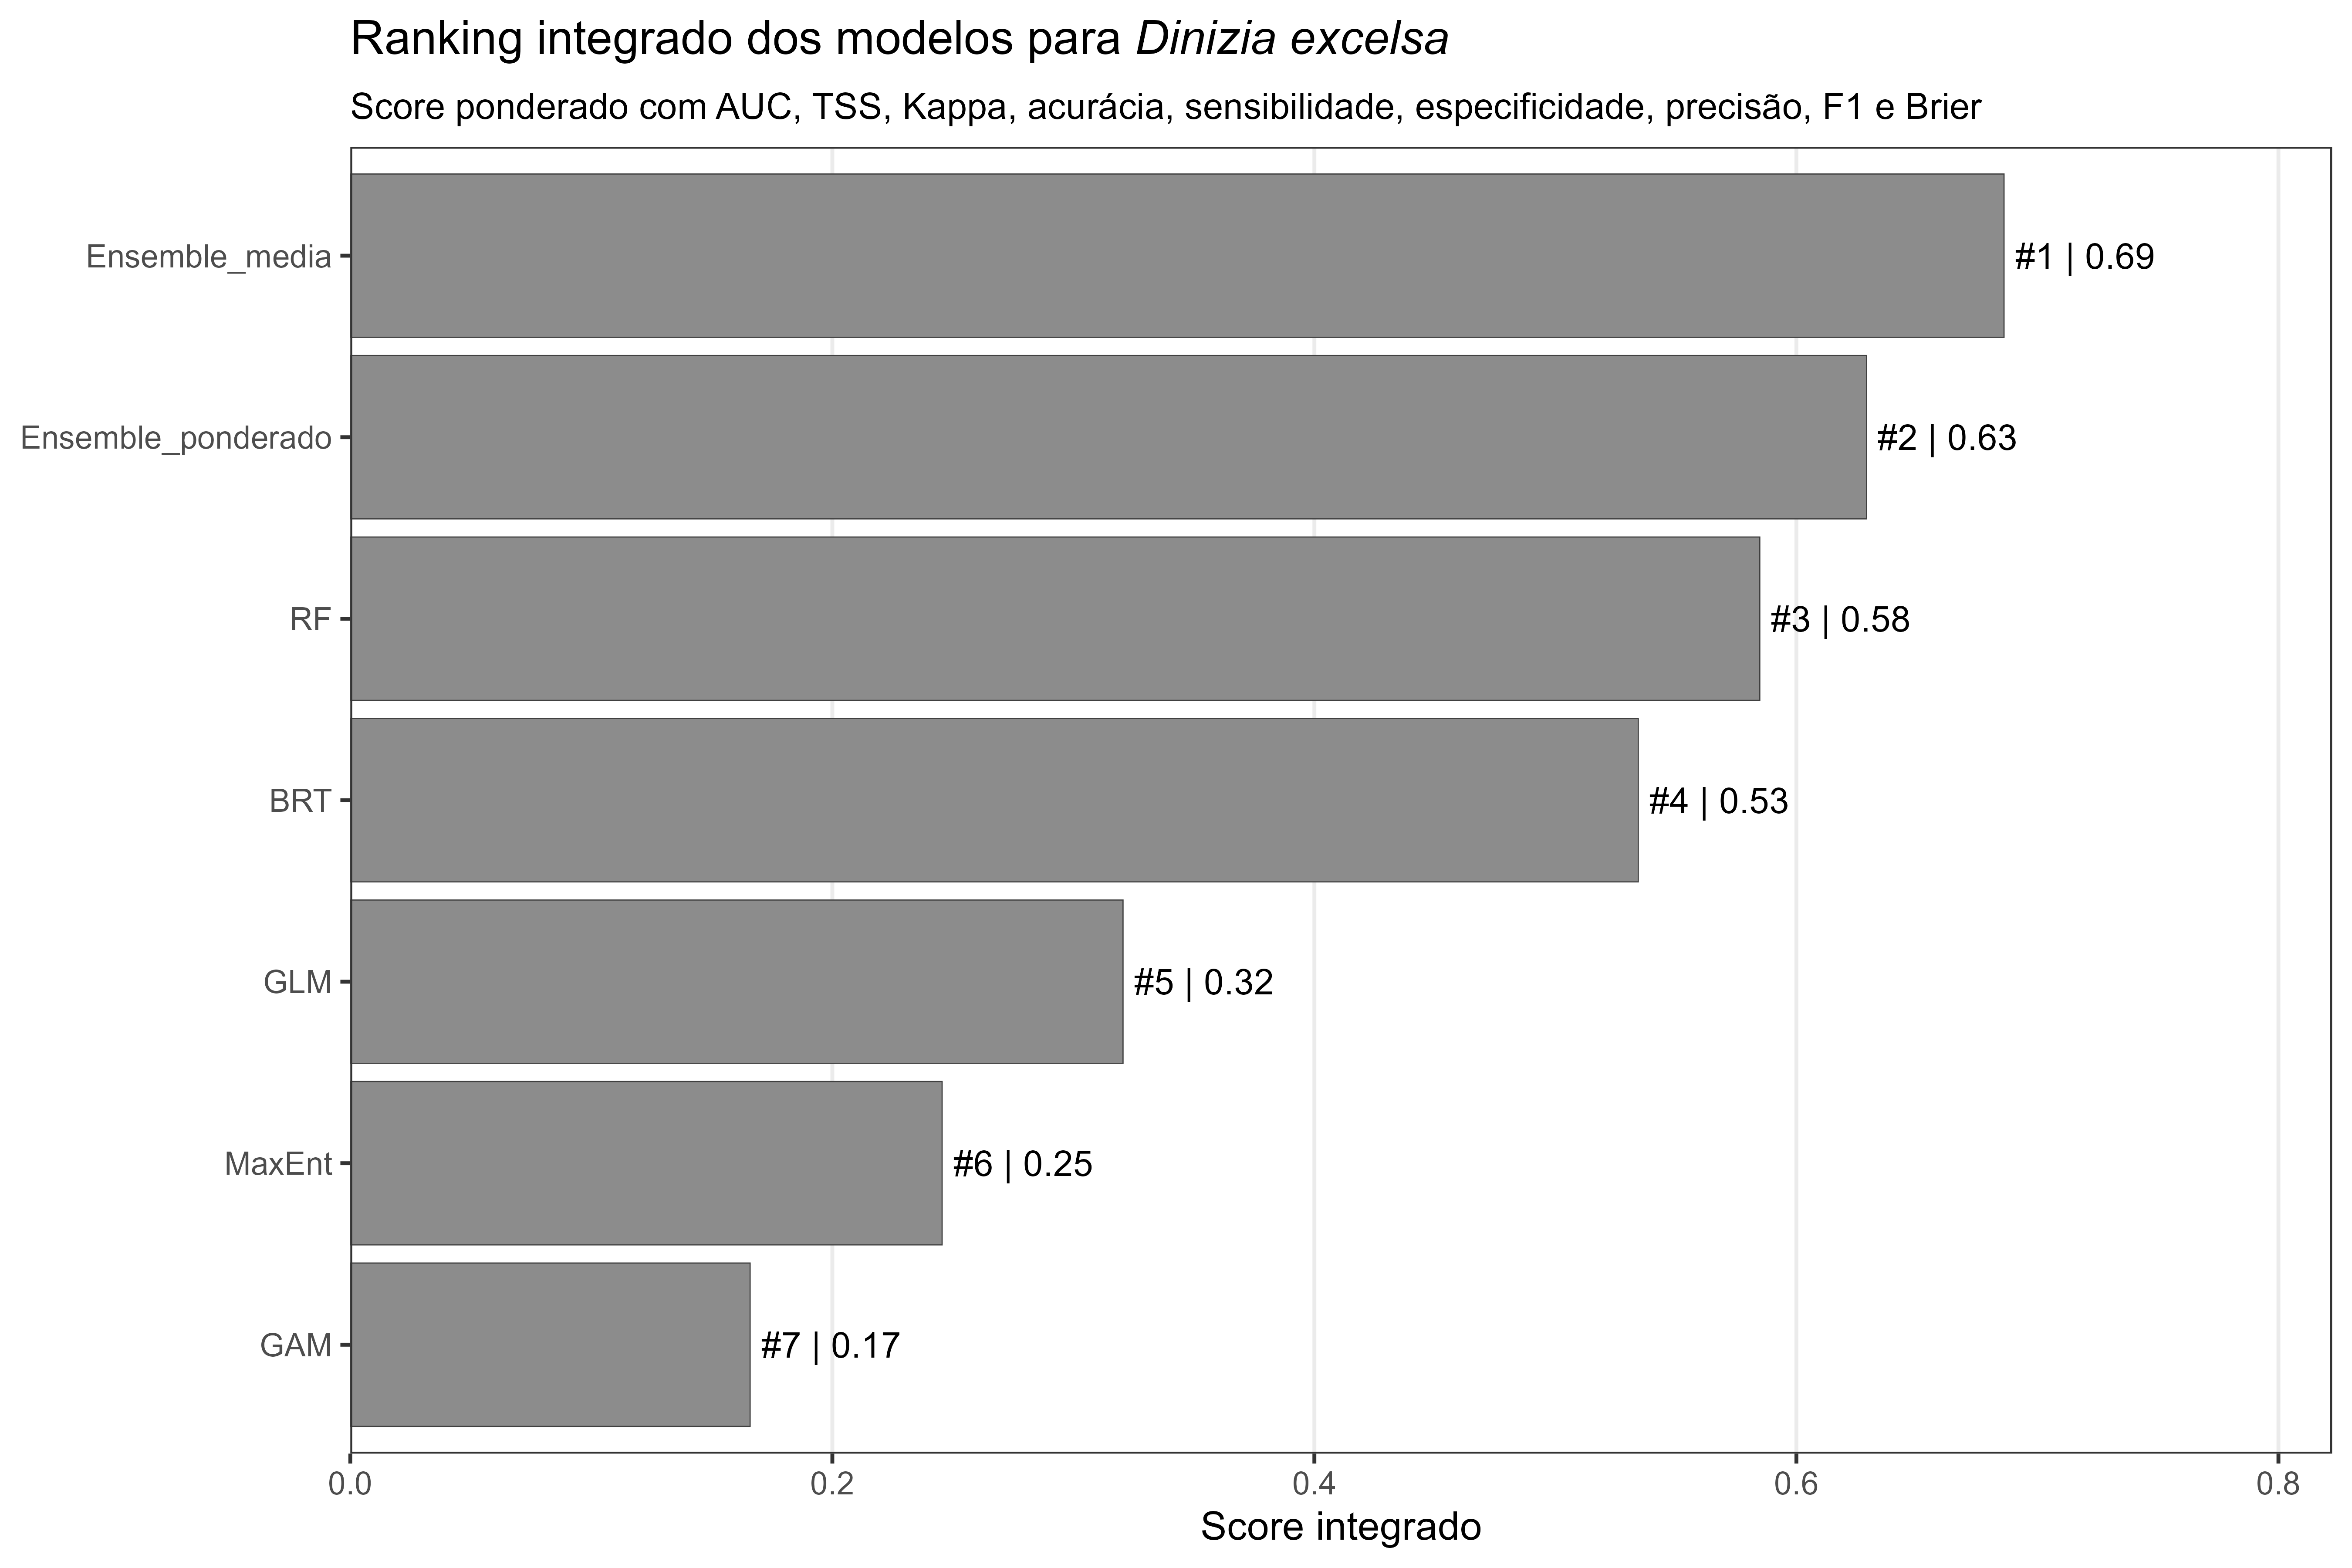
\includegraphics[width=0.95\textwidth]{figuras/unidade12/unidade12_ranking_modelos.png}
	\caption{Ranking comparativo dos modelos considerando AUC, TSS, Kappa, sensibilidade, especificidade e Boyce Index.}
	\label{fig:unidade12_ranking}
\end{figure}

\section{Pipeline completo}

\rscriptfile{scripts/unidade12/08_pipeline_avaliacao.R}

\section{Síntese da unidade}

A avaliação de modelos deve combinar múltiplas métricas, validação independente e interpretação ecológica. Para \textit{Dinizia excelsa}, as métricas ajudam a comparar modelos com diferentes estruturas, mas a decisão final sobre quais modelos utilizar em projeções futuras deve considerar também coerência espacial, curvas de resposta, incerteza e plausibilidade ecológica.

\begin{conceito}[title={\faBook\quad Mensagem central}]
	Nenhuma métrica isolada é suficiente para validar um SDM. A avaliação robusta combina métricas contínuas, métricas binárias, interpretação ecológica e análise espacial das predições.
\end{conceito}

\section{Exercícios de fixação}

\subsection*{A. Conceituais}

\begin{enumerate}
	\item Explique a diferença entre AUC e TSS.
	\item Por que AUC pode ser problemático em dados presença-background?
	\item O que significam sensibilidade e especificidade?
\end{enumerate}

\subsection*{B. Interpretação}

\begin{enumerate}[resume]
	\item Dois modelos apresentam o mesmo AUC, mas sensibilidades muito
	diferentes. Que consequências isso pode ter para a identificação de áreas
	potencialmente adequadas?
	\item Um modelo perde desempenho quando a validação aleatória é substituída
	por blocos espaciais. Interprete esse resultado sem concluir automaticamente
	que o algoritmo é inadequado.
	\item Explique o significado ecológico do Boyce Index e uma limitação dessa
	métrica.
\end{enumerate}

\subsection*{C. Computacionais}

\begin{enumerate}[resume]
	\item Recalcule as métricas usando os mesmos folds para todos os algoritmos e
	compare a variação entre folds, não apenas a média.
	\item Construa uma partição espacial e uma partição ambiental. Compare o
	número de presenças e backgrounds em cada fold e discuta o equilíbrio das
	partições.
	\item Compare pelo menos dois critérios de limiar e quantifique como eles
	alteram área adequada, omissão e comissão.
\end{enumerate}

\subsection*{D. Pensamento crítico}

\begin{enumerate}[resume]
	\item Por que mapas binários devem ser interpretados com cautela?
	\item Como a estratégia de validação deveria mudar entre interpolação na
	Amazônia e projeção para um clima futuro?
	\item Um modelo de presença--background com AUC alto pode ser descrito como
	modelo bem calibrado de probabilidade de ocorrência? Justifique.
\end{enumerate}

\subsection*{Mini-projeto}

Escolha um dos algoritmos ajustados para \textit{Dinizia excelsa}. Compare sua
avaliação sob partição aleatória e sob blocos espaciais, mantendo dados,
preditores e métricas constantes. Apresente o mapa dos folds, a distribuição das
distâncias treino--teste, as métricas por fold e uma recomendação sobre o uso do
modelo para interpolação e transferência.

% ============================================================
% UNIDADE 13
% ============================================================
